%!TEX root = ../../main.tex

\section{Additional Figures and Tables} % (fold)
\label{app:supplementary}

% XXX Move all graphs and tables here

% Threshold 
\begin{figure}[H]
  \centering
  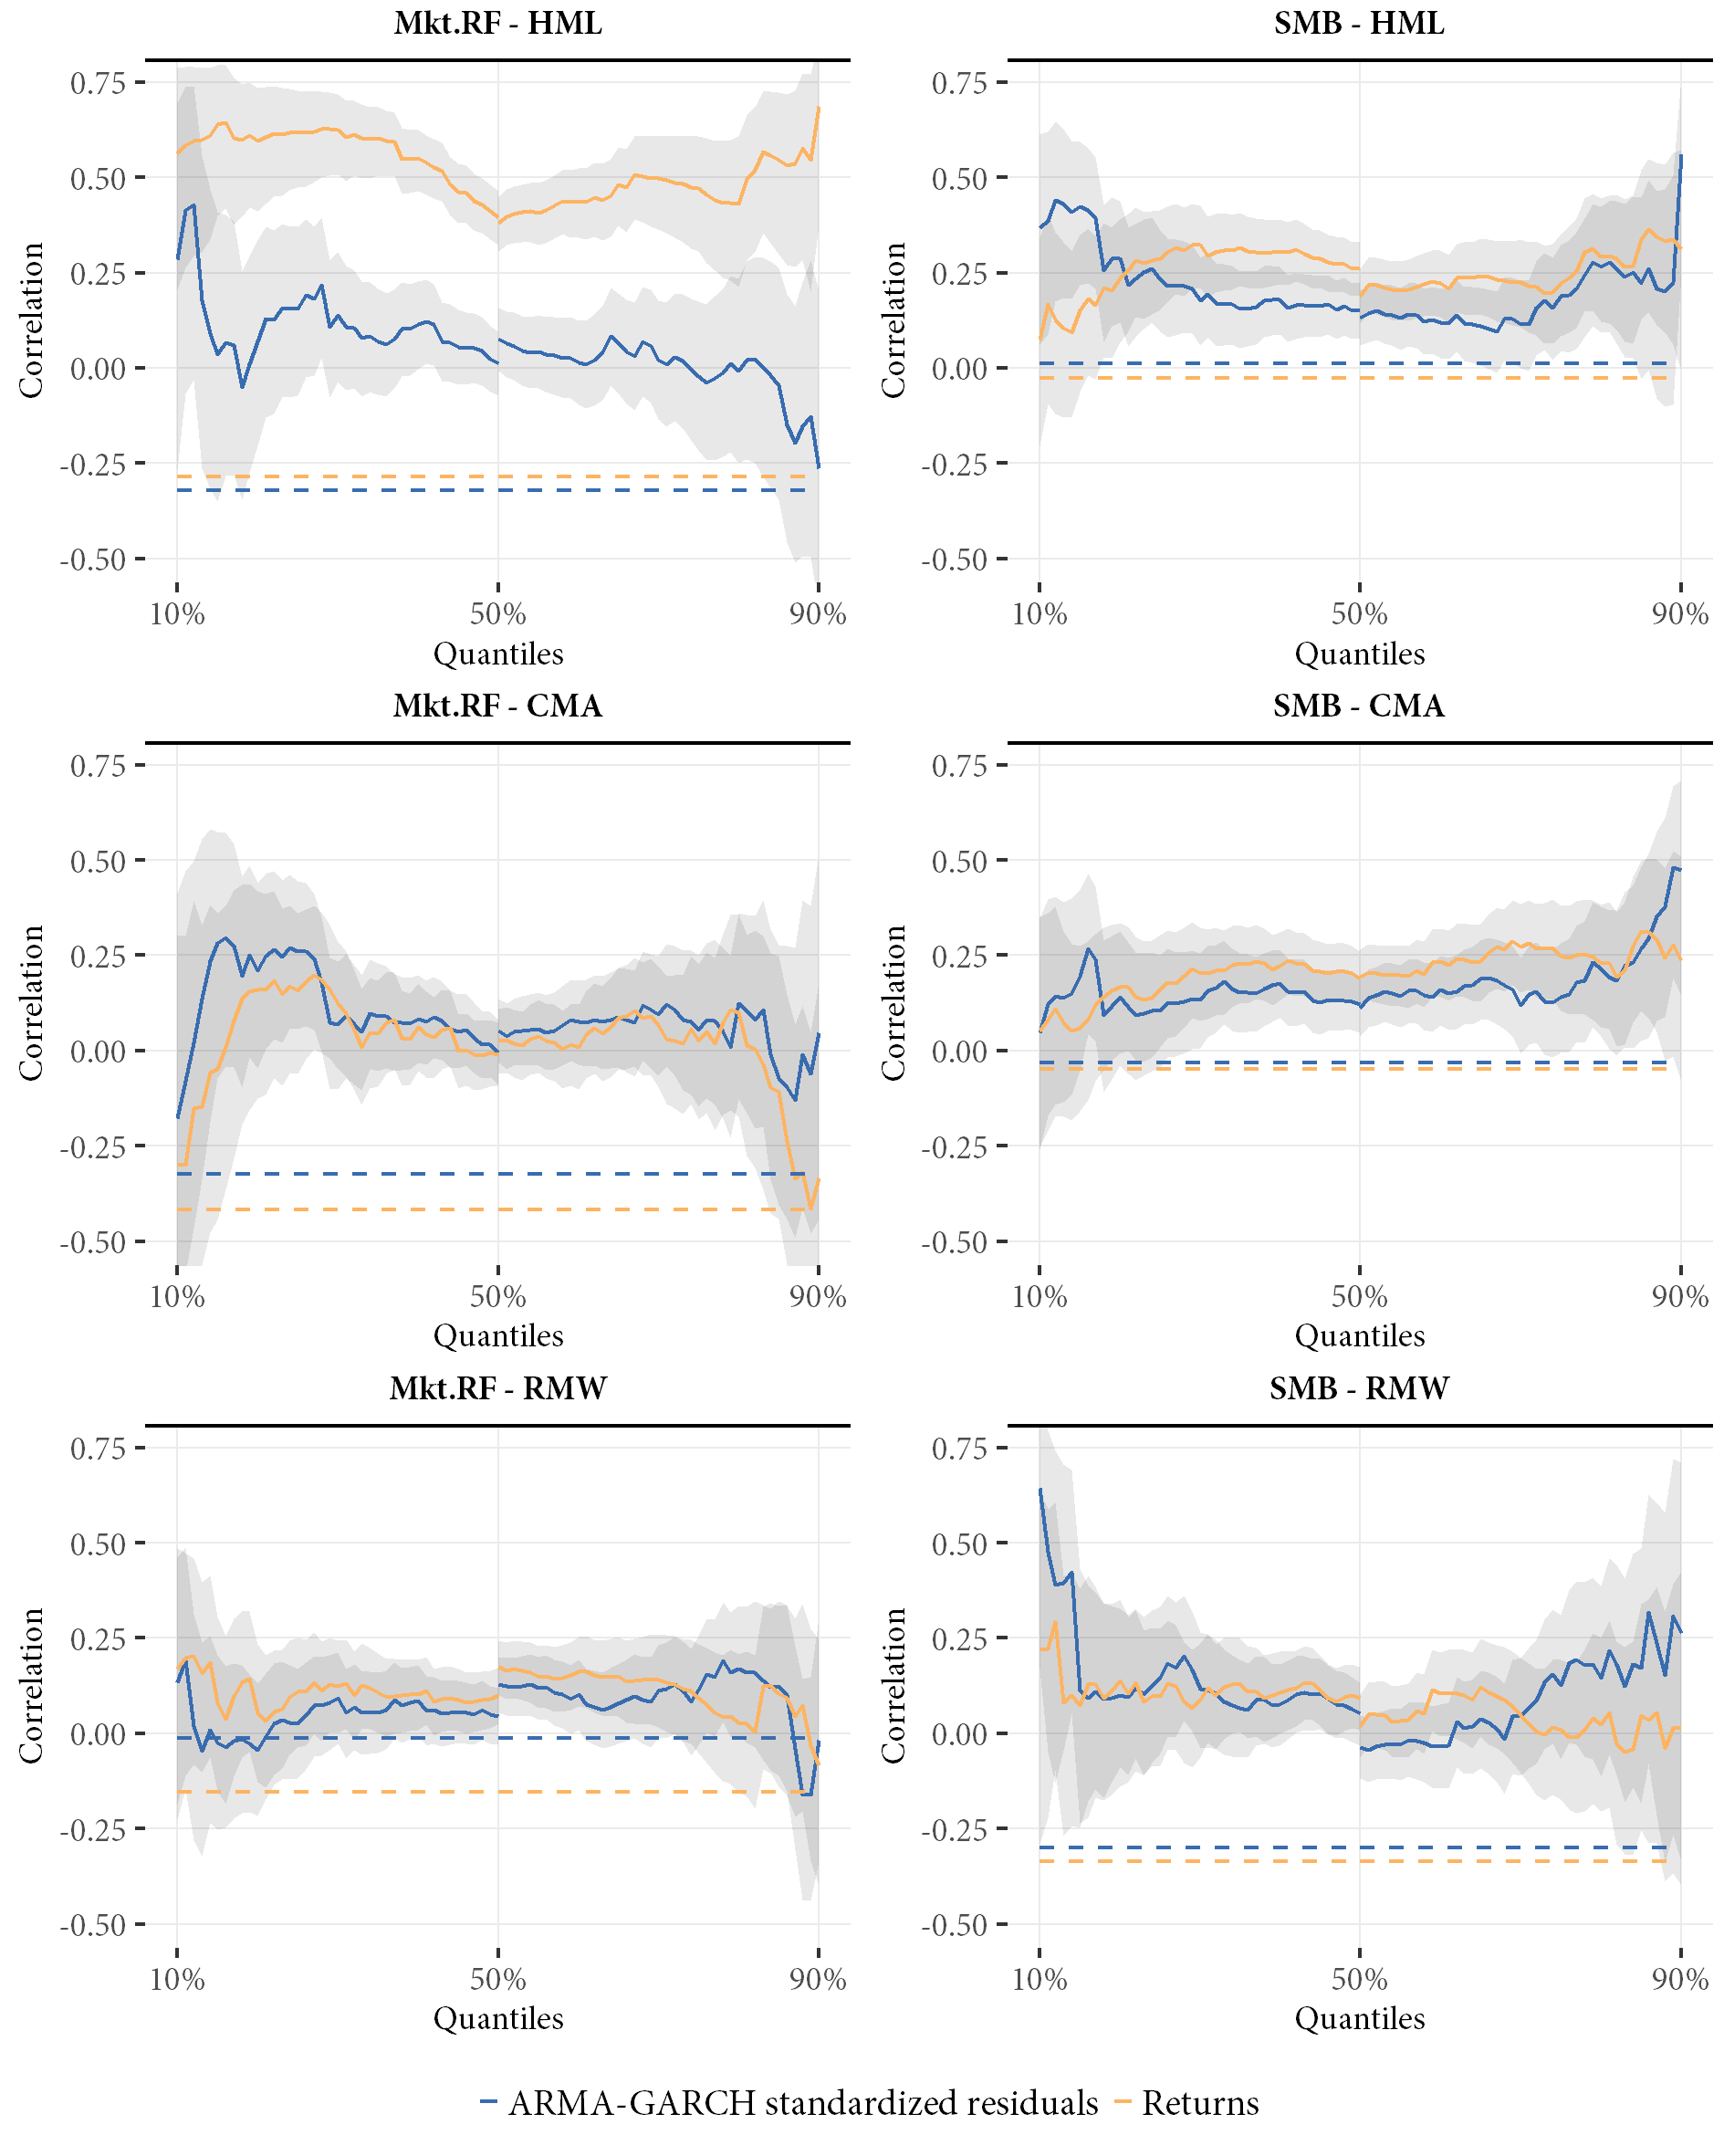
\includegraphics[scale=1]{graphics/appendix_threshold_1.png}
  \footnotesize
  \caption{Threshold correlations of returns and ARMA-GARCH standardized residuals}
  \begin{longcaption}
    Based on weekly data 1963--2016. The formula for threshold correlations for a threshold $p$ is given in~\autoref{eq:th_corr}. 95\% shaded confidence bounds, taking the model as given for standardized residuals. The unconditional correlations are given by the dashed lines.
  \end{longcaption}
  \label{fig:appendix_threshold1}
\end{figure}
\begin{figure}[H]
  \ContinuedFloat
  \centering
  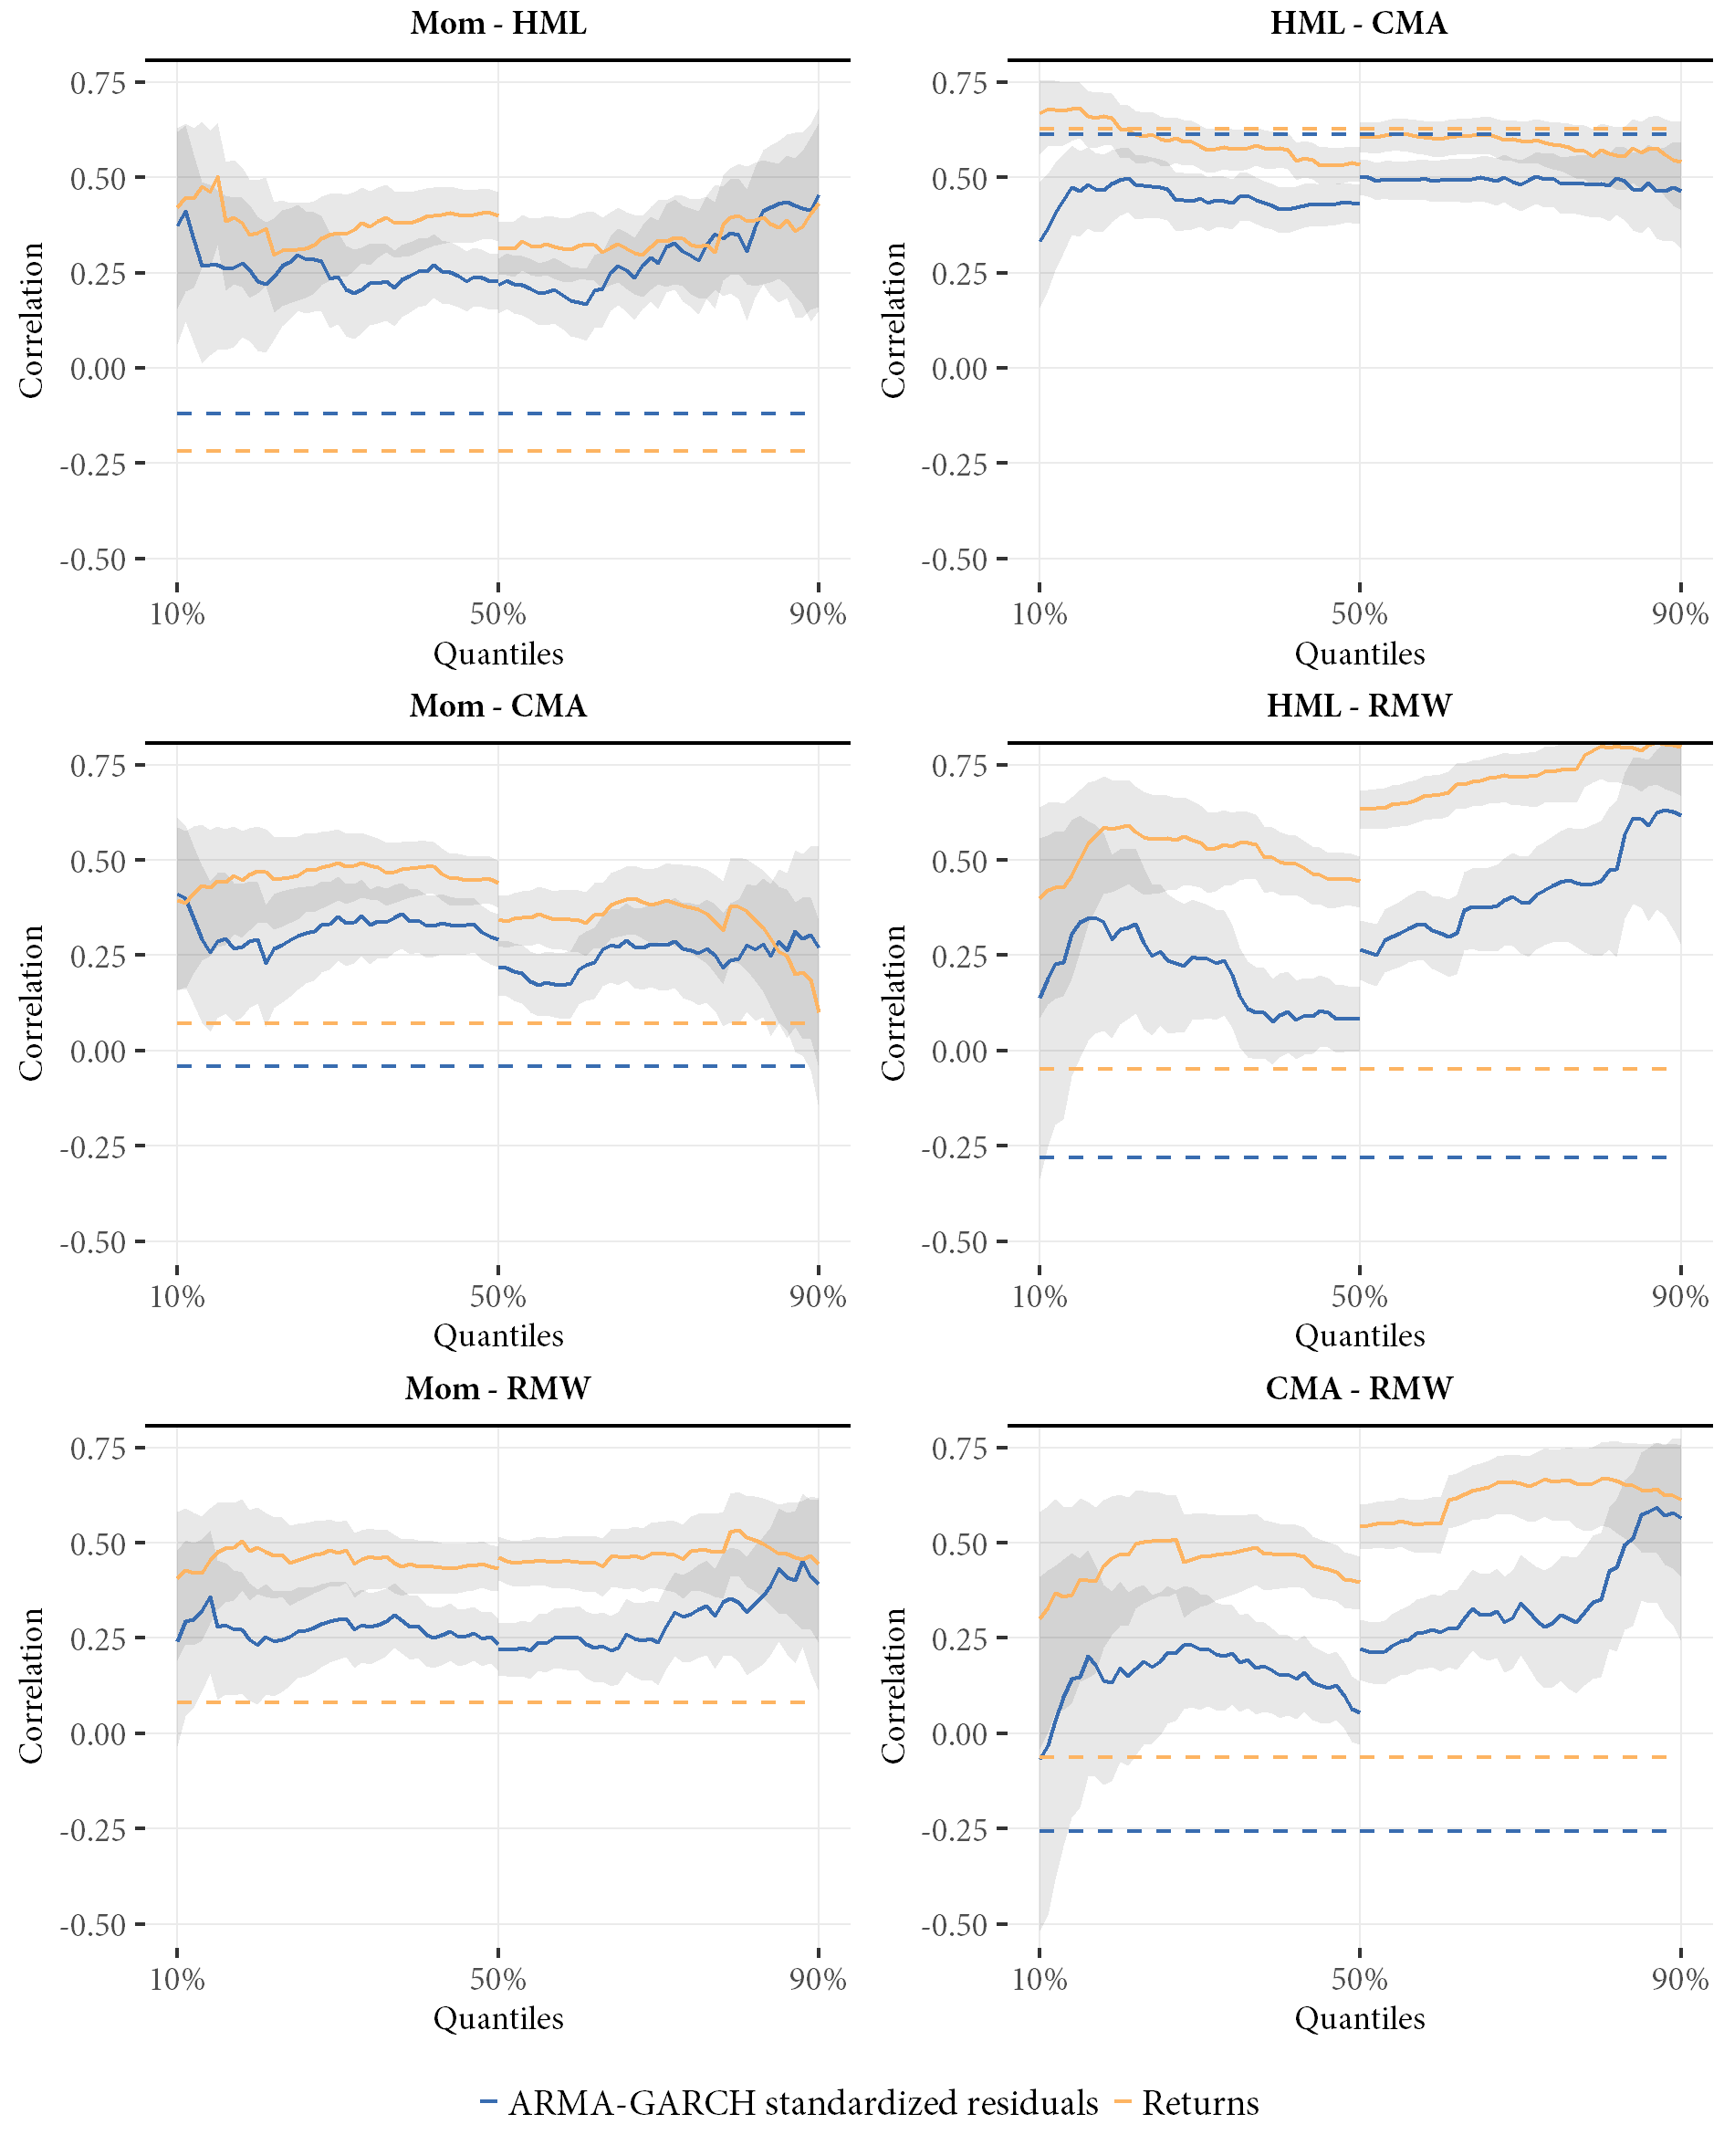
\includegraphics[scale=1]{graphics/appendix_threshold_2.png}
  \footnotesize
  \caption{Threshold correlations of returns and ARMA-GARCH standardized residuals (cont.)}
\end{figure}

% Rolling on returns
\begin{figure}[!ht]
  \centering
  \footnotesize
  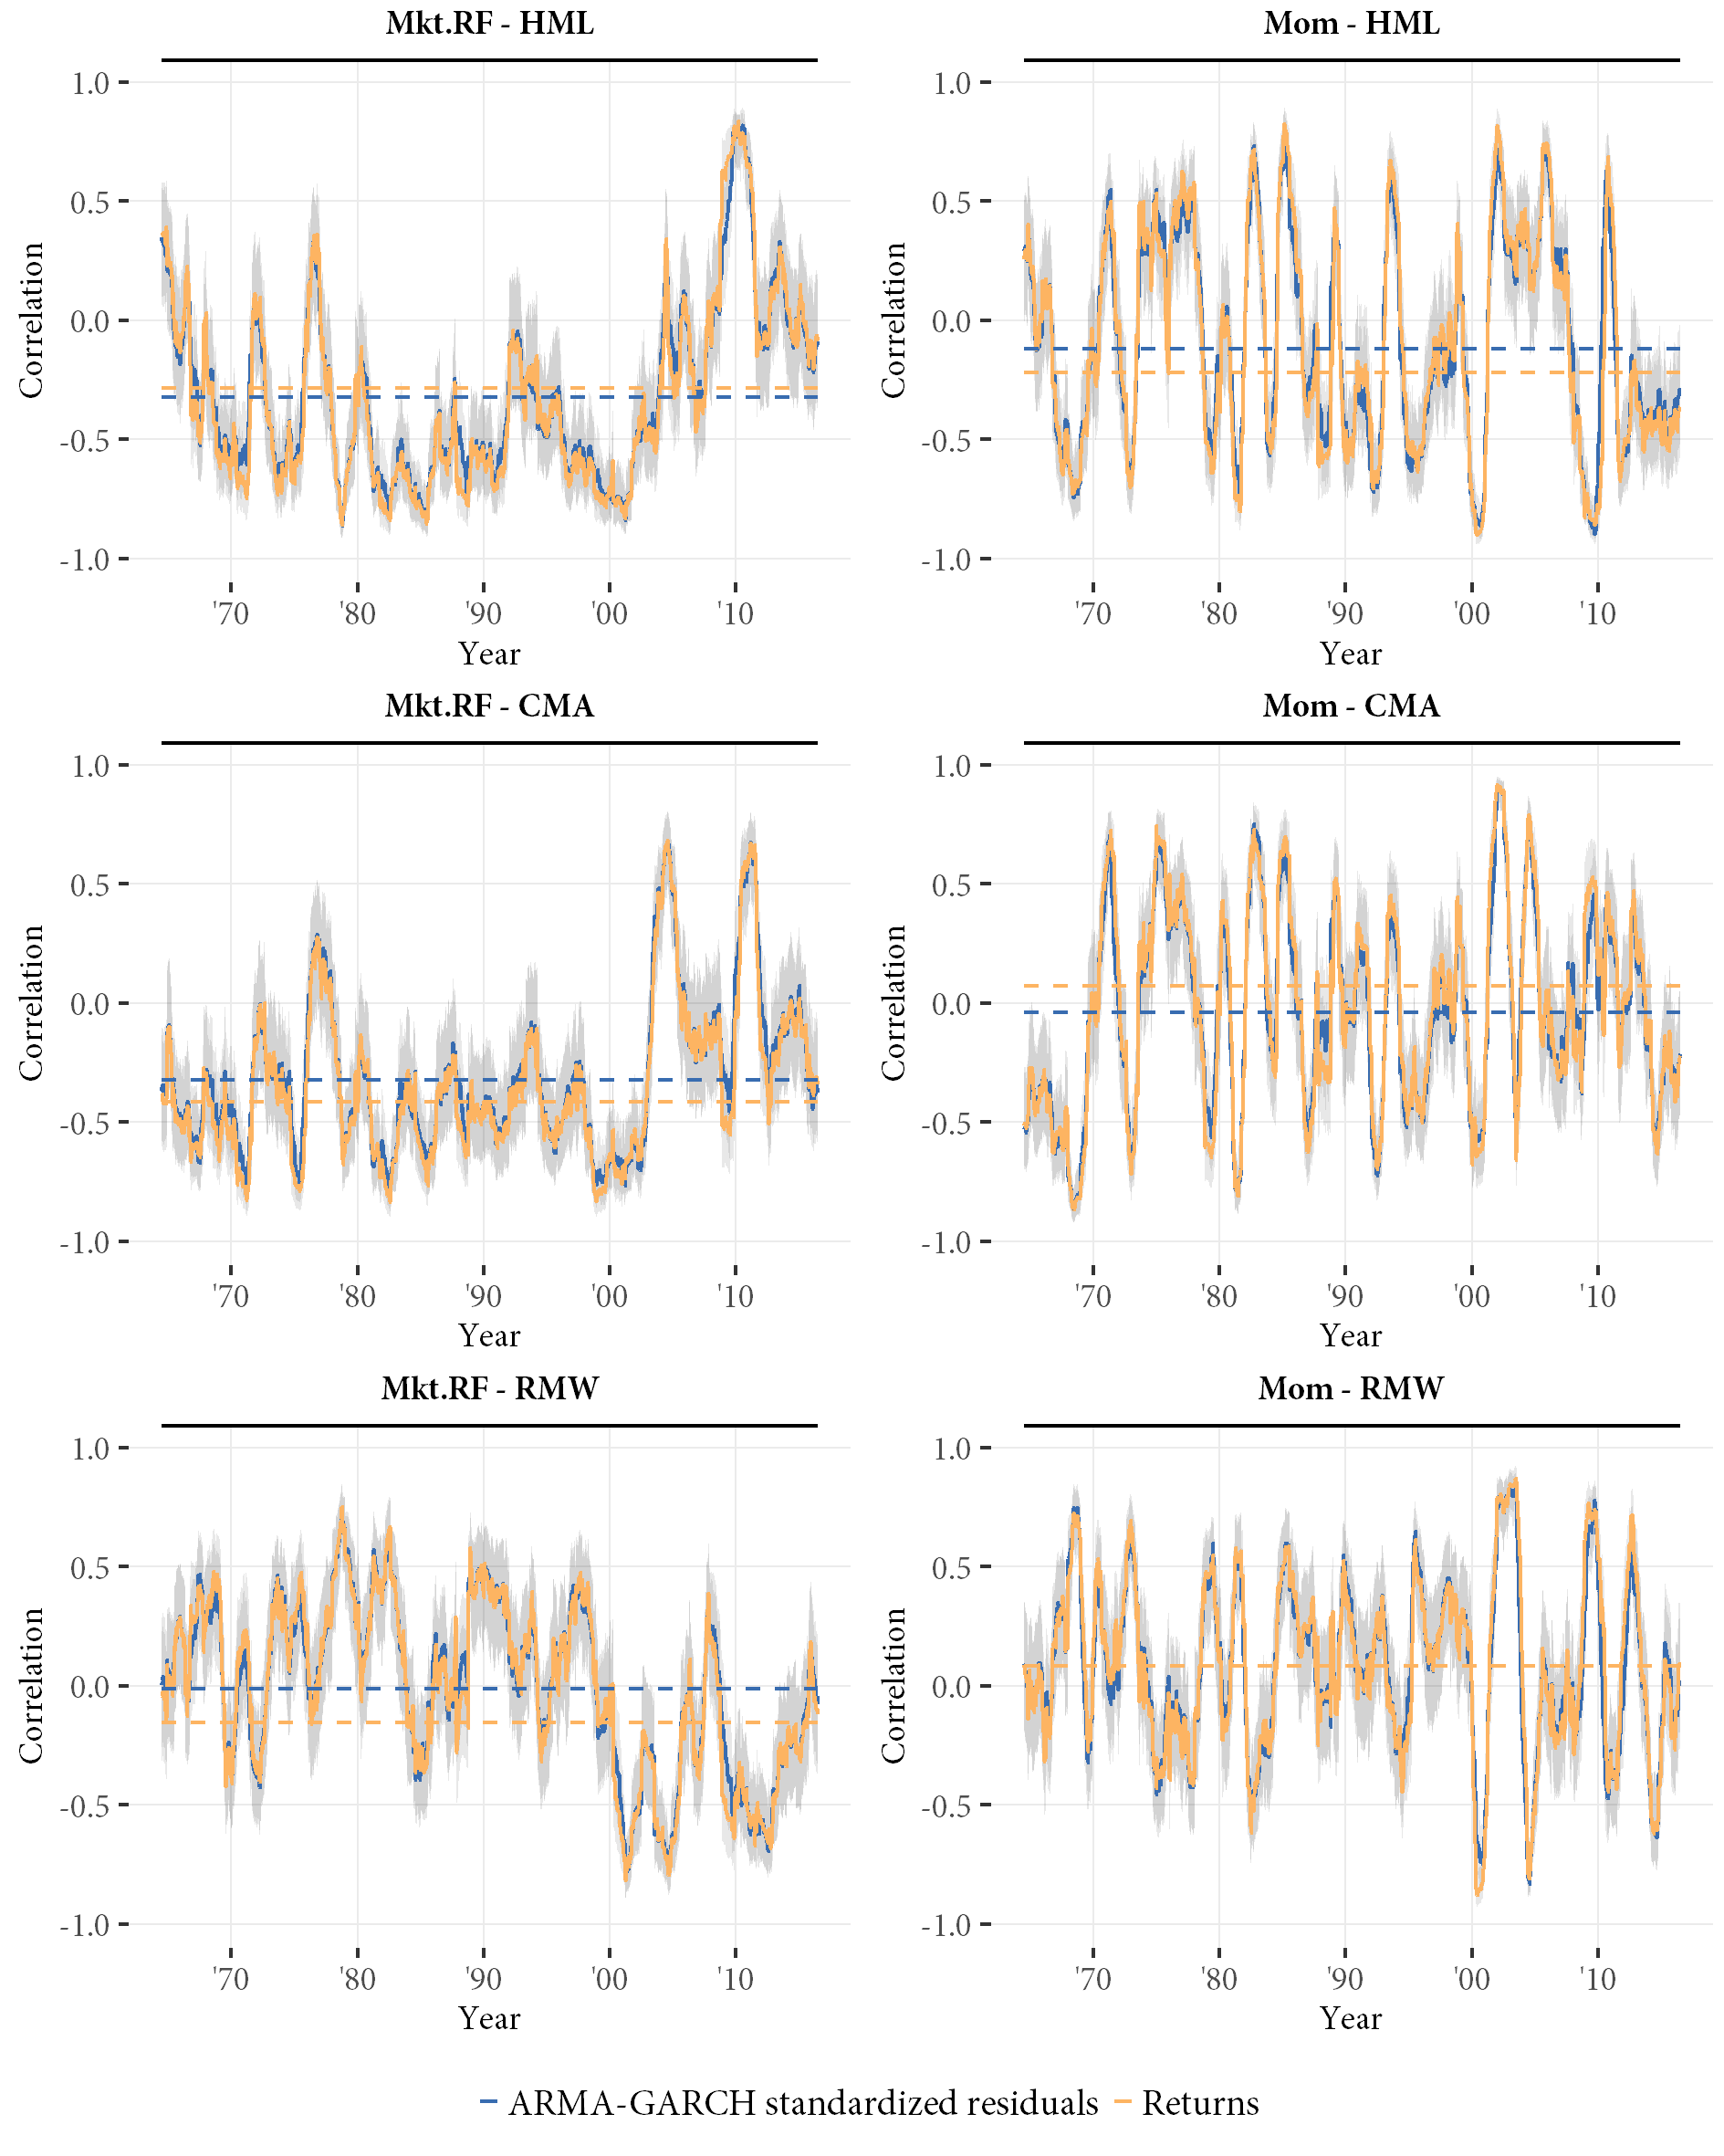
\includegraphics[scale=1]{graphics/appendix_rolling1.png}
  
  \caption{Rolling correlations of returns and ARMA-GARCH standardized residuals}
  \begin{longcaption}
    Based on weekly data 1963--2016. 95\% shaded confidence bounds, taking the model as given for standardized residuals. The unconditional correlations are given by the dashed lines.
  \end{longcaption}
  \label{fig:appendix_rolling1}
\end{figure}
\begin{figure}[!ht]
  \ContinuedFloat
  \centering
  \footnotesize
  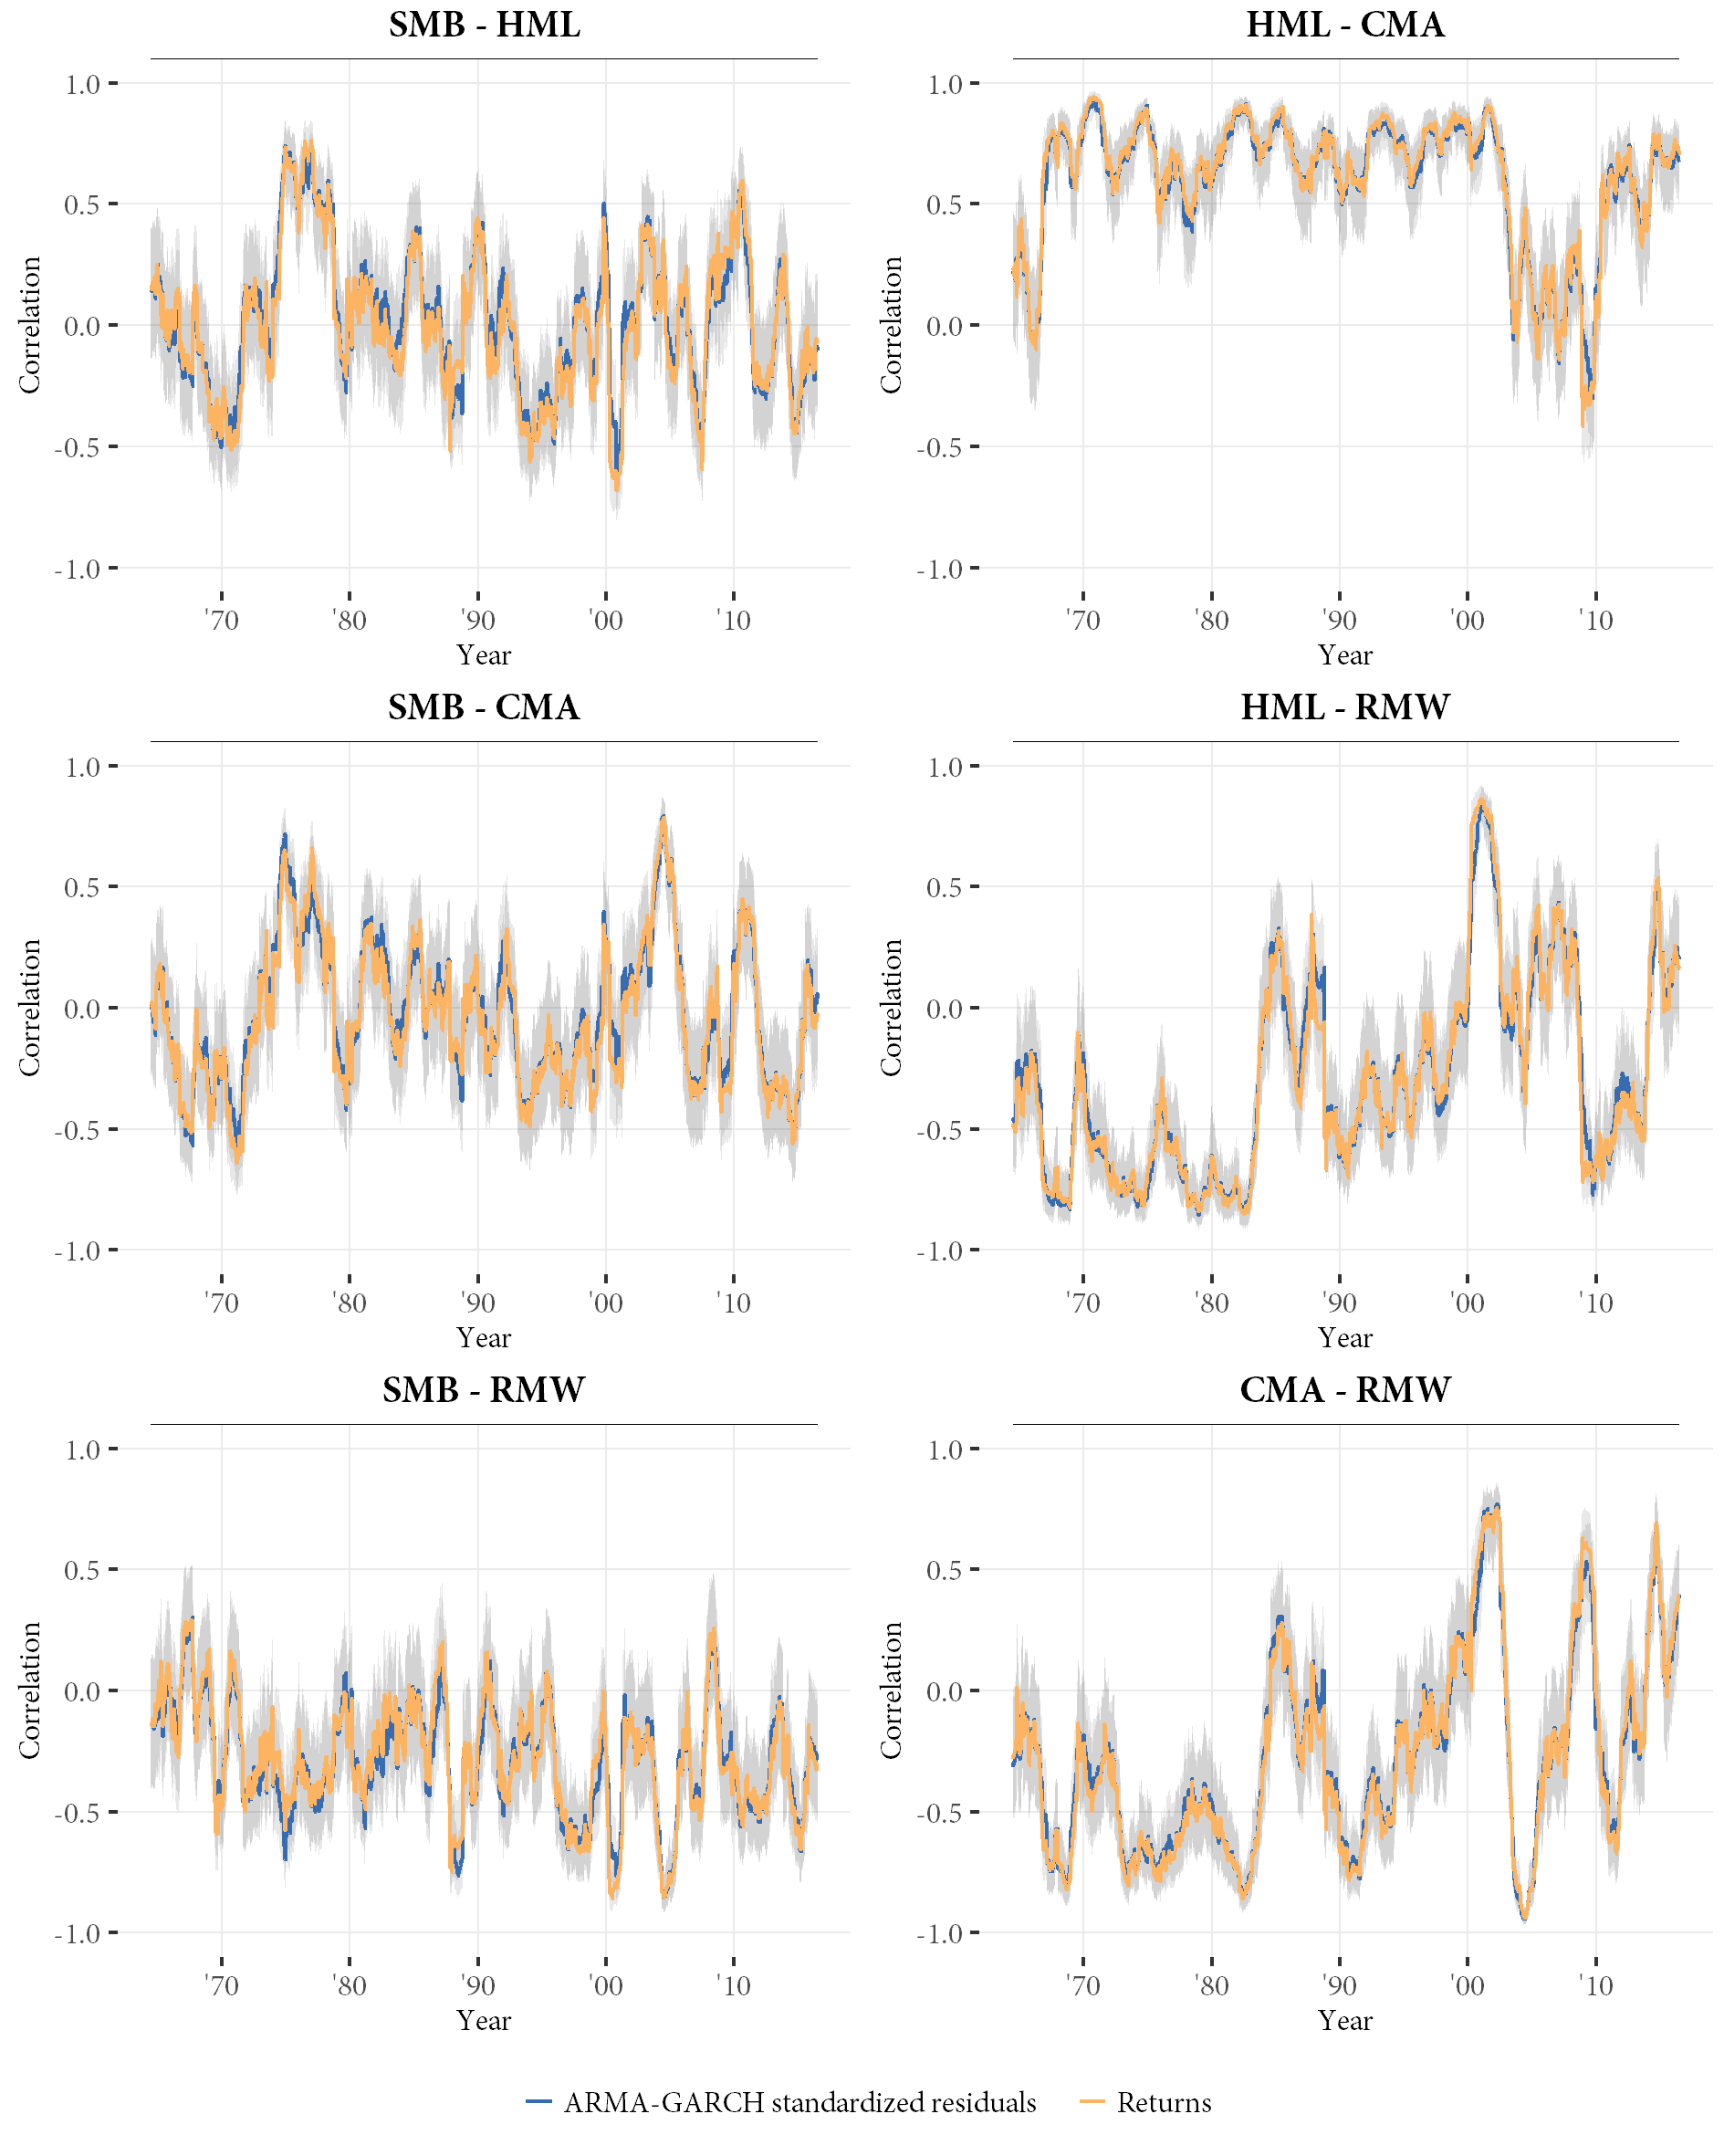
\includegraphics[scale=1]{graphics/appendix_rolling2.png}

  \caption{Rolling correlations of returns and ARMA-GARCH standardized residuals (cont.)}
\end{figure}

% MV performance table
%!TEX root = ../../main.tex

\begin{table}
  \centering
  \footnotesize
  \renewcommand{\arraystretch}{1.2}

  \caption{Mean-Variance optimization with static sample inputs (1963--2016)}

  \begin{longcaption}
    Static weights are the MV optimal weights based on in-sample sample estimators of means and covariances. Differences in average weights are expressed relative to the full five- and six-factor models. Performance measures are based on realized returns. SR is the annualized Sharpe Ratio. VaR, ES and CDB are all based on the one-week-ahead 5\% lower tail of the return distribution, which is given by simulations from the copula model. Differences in CDB are to be read as column model minus row model and its associated standard errors (in parentheses) are computed taking the copula model as given.
  \end{longcaption}

  \label{tab:mw_mv_sample}

  \begin{tabularx}{\textwidth}{@{} l dddd X dddd @{}}
    \toprule
    &
      \multicolumn{4}{c}{Five (four) factor models} &&
      \multicolumn{4}{c}{Six (five) factor models} \\
    \cmidrule{2-5}
    \cmidrule{7-10}
    &
      \multirow{2}{*}{All} &
      \multicolumn{1}{c}{Excl.} &
      \multicolumn{1}{c}{Excl.} &
      \multicolumn{1}{c}{Excl.} & &
      \multirow{2}{*}{All} &
      \multicolumn{1}{c}{Excl.} &
      \multicolumn{1}{c}{Excl.} &
      \multicolumn{1}{c}{Excl.} \\
    &
      &
      \multicolumn{1}{c}{HML} &
      \multicolumn{1}{c}{CMA} &
      \multicolumn{1}{c}{RMW} &&
      &
      \multicolumn{1}{c}{HML} &
      \multicolumn{1}{c}{CMA} &
      \multicolumn{1}{c}{RMW} \\
    \midrule
    \multicolumn{1}{@{}l}{\textbf{Static weights}} \\
    Mkt.RF & 13.6 & 13.7 & 13.8 & 21.5 & & 13.2 & 13.4 & 13.2 & 18.5 \\
    SMB    & 14.0 & 14.1 & 18.0 & 12.0 & & 12.0 & 12.7 & 13.4 & 9.1 \\
    HML    & 6.2  &      & 26.7 & 11.2 & & 13.2 &      & 27.0 & 22.3 \\
    CMA    & 33.2 & 39.0 &      & 55.3 & & 22.2 & 35.2 &      & 29.2 \\
    RMW    & 33.0 & 33.2 & 41.5 &      & & 27.7 & 29.0 & 30.2 & \\
    Mom    &      &      &      &      & & 11.7 & 9.7  & 16.2 & 21.0 \\
    \midrule
    \multicolumn{1}{@{}l}{\textbf{Difference weights}} \\
    Mkt.RF & & 0.1  & 0.2   & 7.9   & & & 0.2   & 0.0   & 5.3 \\
    SMB    & & 0.2  & 4.0   & -2.0  & & & 0.7   & 1.4   & -2.9 \\
    HML    & & -6.2 & 20.5  & 5.0   & & & -13.2 & 13.7  & 9.1 \\
    CMA    & & 5.8  & -33.2 & 22.1  & & & 13.0  & -22.2 & 7.0 \\
    RMW    & & 0.3  & 8.5   & -33.0 & & & 1.4   & 2.6   & -27.7     \\
    Mom    & &      &       &       & & & -2.0  & 4.5   & 9.3 \\
    \midrule
    \multicolumn{1}{@{}l}{\textbf{Performance}} \\
    Mean (\%)      & 3.71  & 3.68  & 3.72  & 4.14  & & 4.32  & 4.14 & 4.56  & 5.10 \\
    SD (\%)        & 2.93  & 2.94  & 3.46  & 4.32  & & 2.99  & 2.99 & 3.35  & 4.19 \\
    SR             & 1.27  & 1.25  & 1.07  & 0.96  & & 1.44  & 1.38 & 1.36  & 1.22 \\
    Avg. VaR  (\%) & 0.56  & 0.57  & 0.63  & 0.89  & & 0.57  & 0.59 & 0.64  & 0.84 \\
    Avg. ES  (\%)  & 0.76  & 0.78  & 0.86  & 1.20  & & 0.79  & 0.81 & 0.88  & 1.16 \\
    Avg. CDB       & 87.34  & 86.68  & 86.45  & 79.15  & & 87.87  & 87.02 & 86.77  & 82.63 \\
    \midrule
    \multicolumn{1}{@{}l}{\textbf{Difference CDB (column model minus row model)}} \\
    All       & & -0.66   & -0.89  & -8.19  & & & -0.85  & -1.10  & -5.24 \\
              & & (0.01) & (0.05) & (0.13) & & & (0.03) & (0.04) & (0.10) \\
    Excl. HML & &        & -0.22  & -7.53  & & &        & -0.22   & -4.40 \\
              & &        & (0.06) & (0.13) & & &        & (0.06) & (0.11) \\
    Excl. CMA & &        &        & -7.31  & & &        &        & -4.14 \\
              & &        &        & (0.14) & & &        &        & (0.10) \\
    \bottomrule
  \end{tabularx}
\end{table}


% Weights of CDB portfolios over time
\begin{figure}[htbp]
  \centering
  \footnotesize
  \begin{subfigure}{0.45\textwidth}
    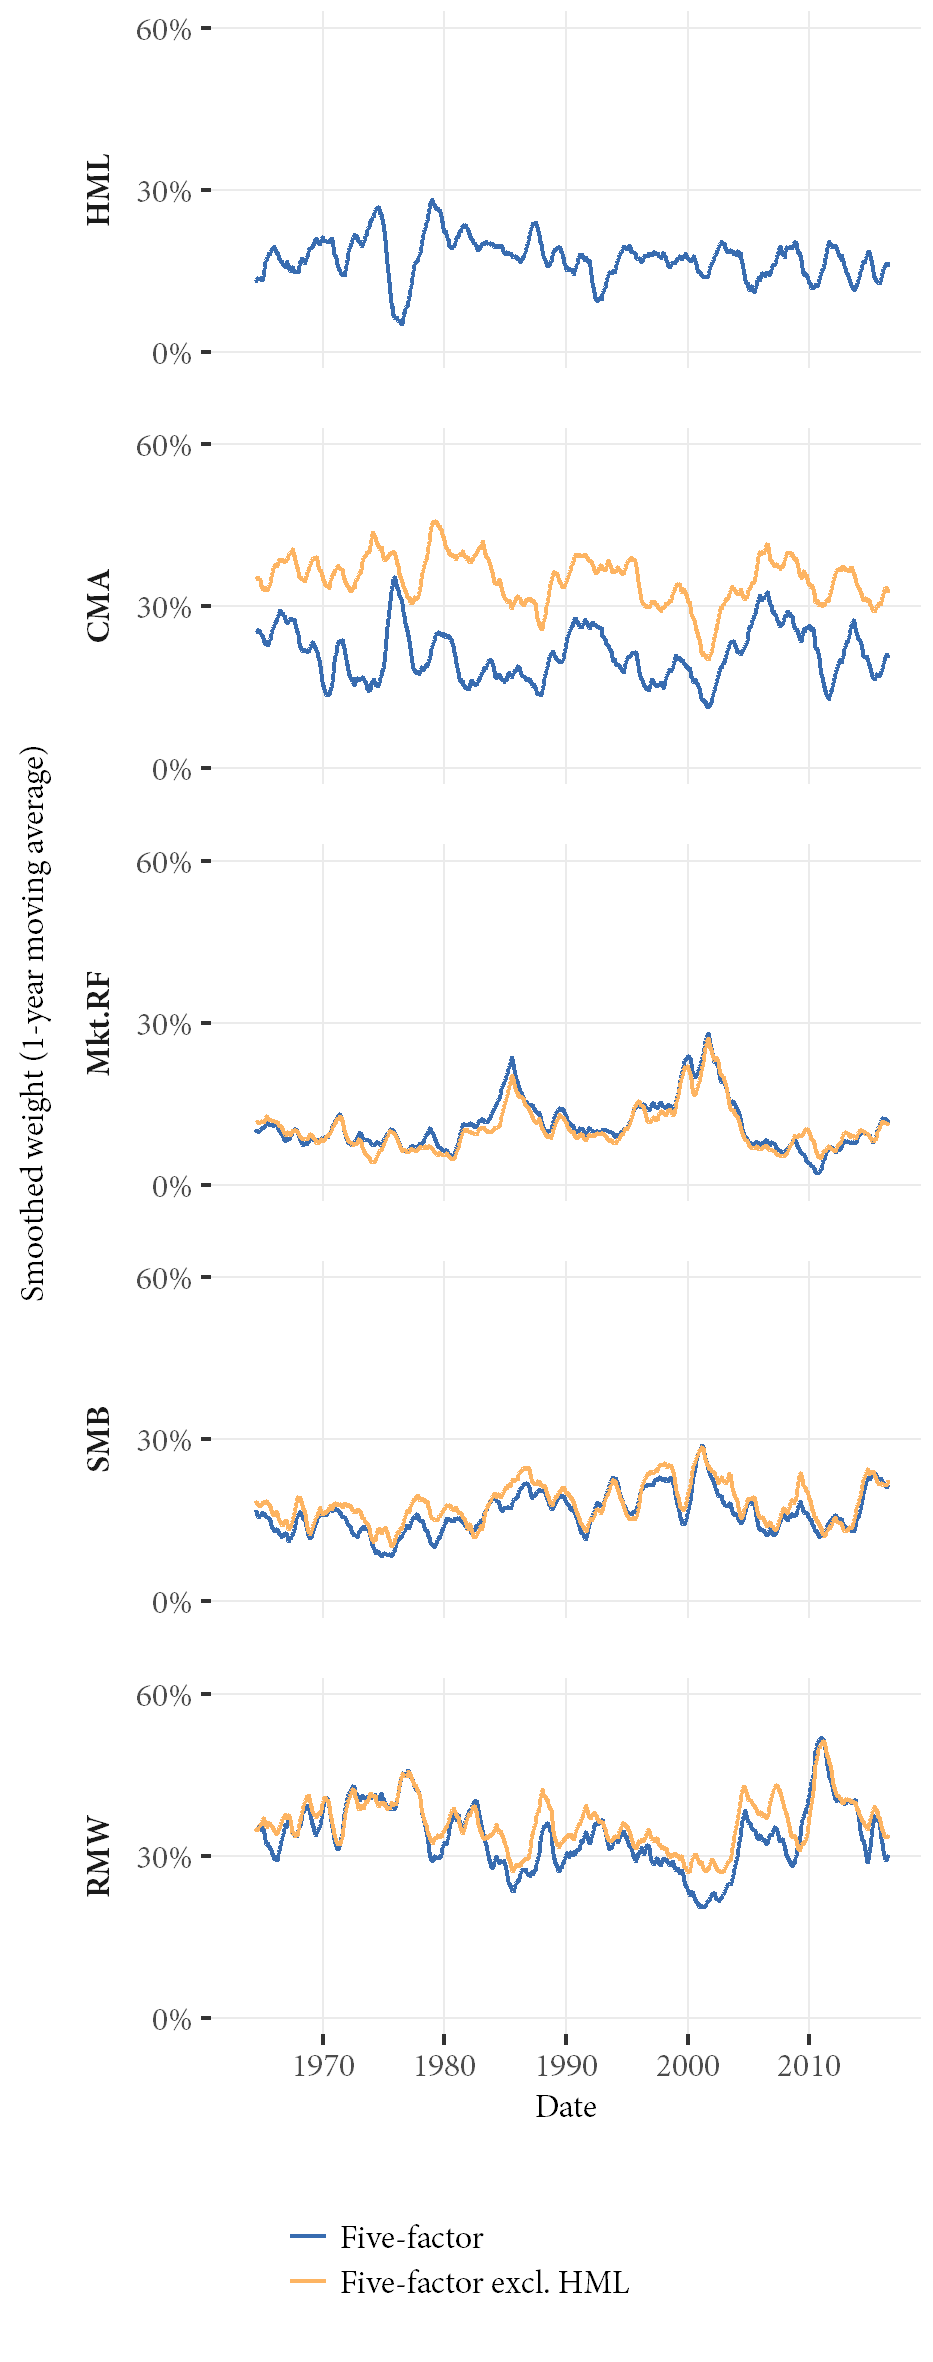
\includegraphics[width=\textwidth]{graphics/weights/appendix_Weights_CDB_5F_EXCL_HML_5F.png}
    \caption{Excluding HML}
  \end{subfigure}
  ~
  \begin{subfigure}{0.45\textwidth}
    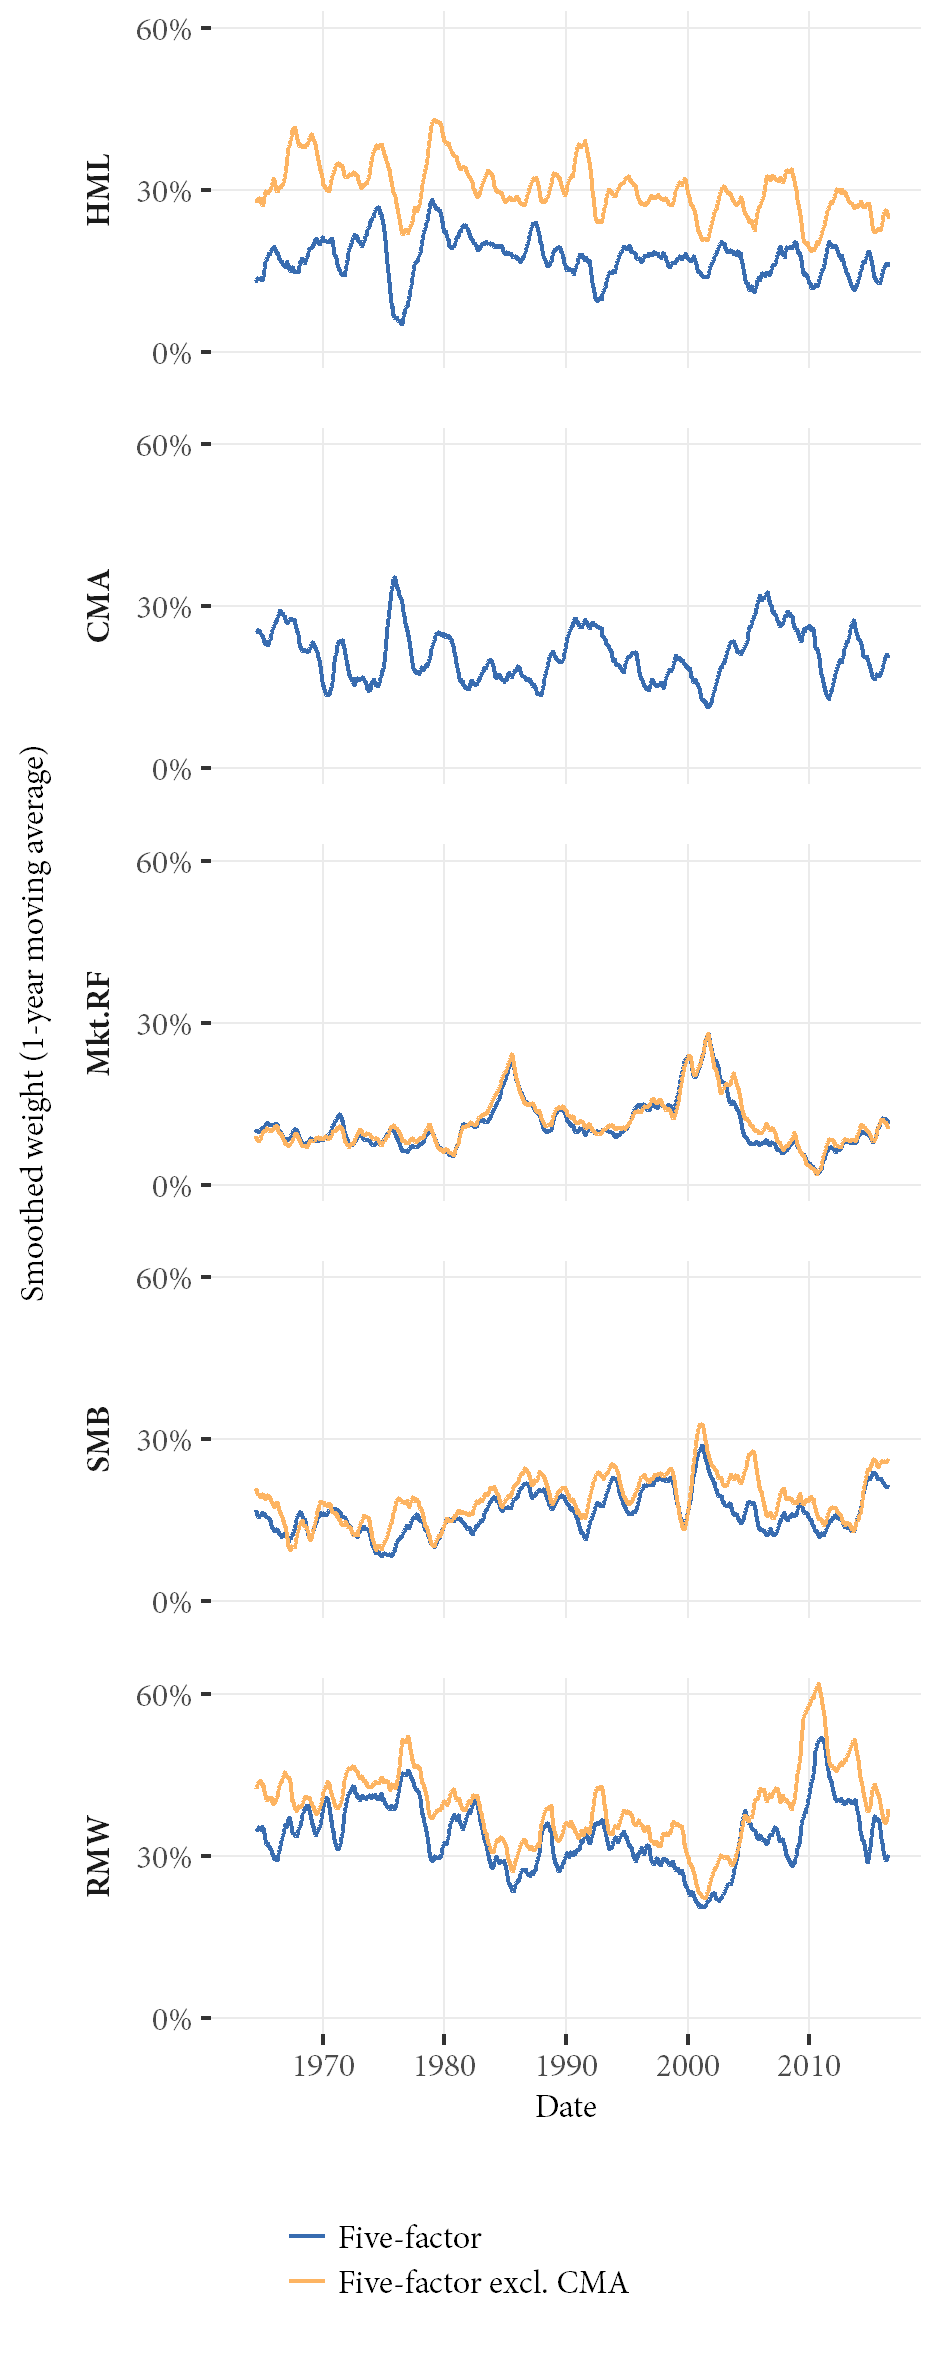
\includegraphics[width=\textwidth]{graphics/weights/appendix_Weights_CDB_5F_EXCL_CMA_5F.png}
    \caption{Excluding CMA}
  \end{subfigure}  
  \caption{CDB optimal weights with five factors}
  \label{fig:cdb_optimal_5}

  \begin{longcaption}
    Smoothed as 1-year moving averages. Left hand panel including and excluding HML, right hand including and excluding CMA. Based on one-week-ahead forecasts from the copula model 1963--2016.
  \end{longcaption}
\end{figure}

\begin{figure}[htbp]
  \ContinuedFloat
  \centering
  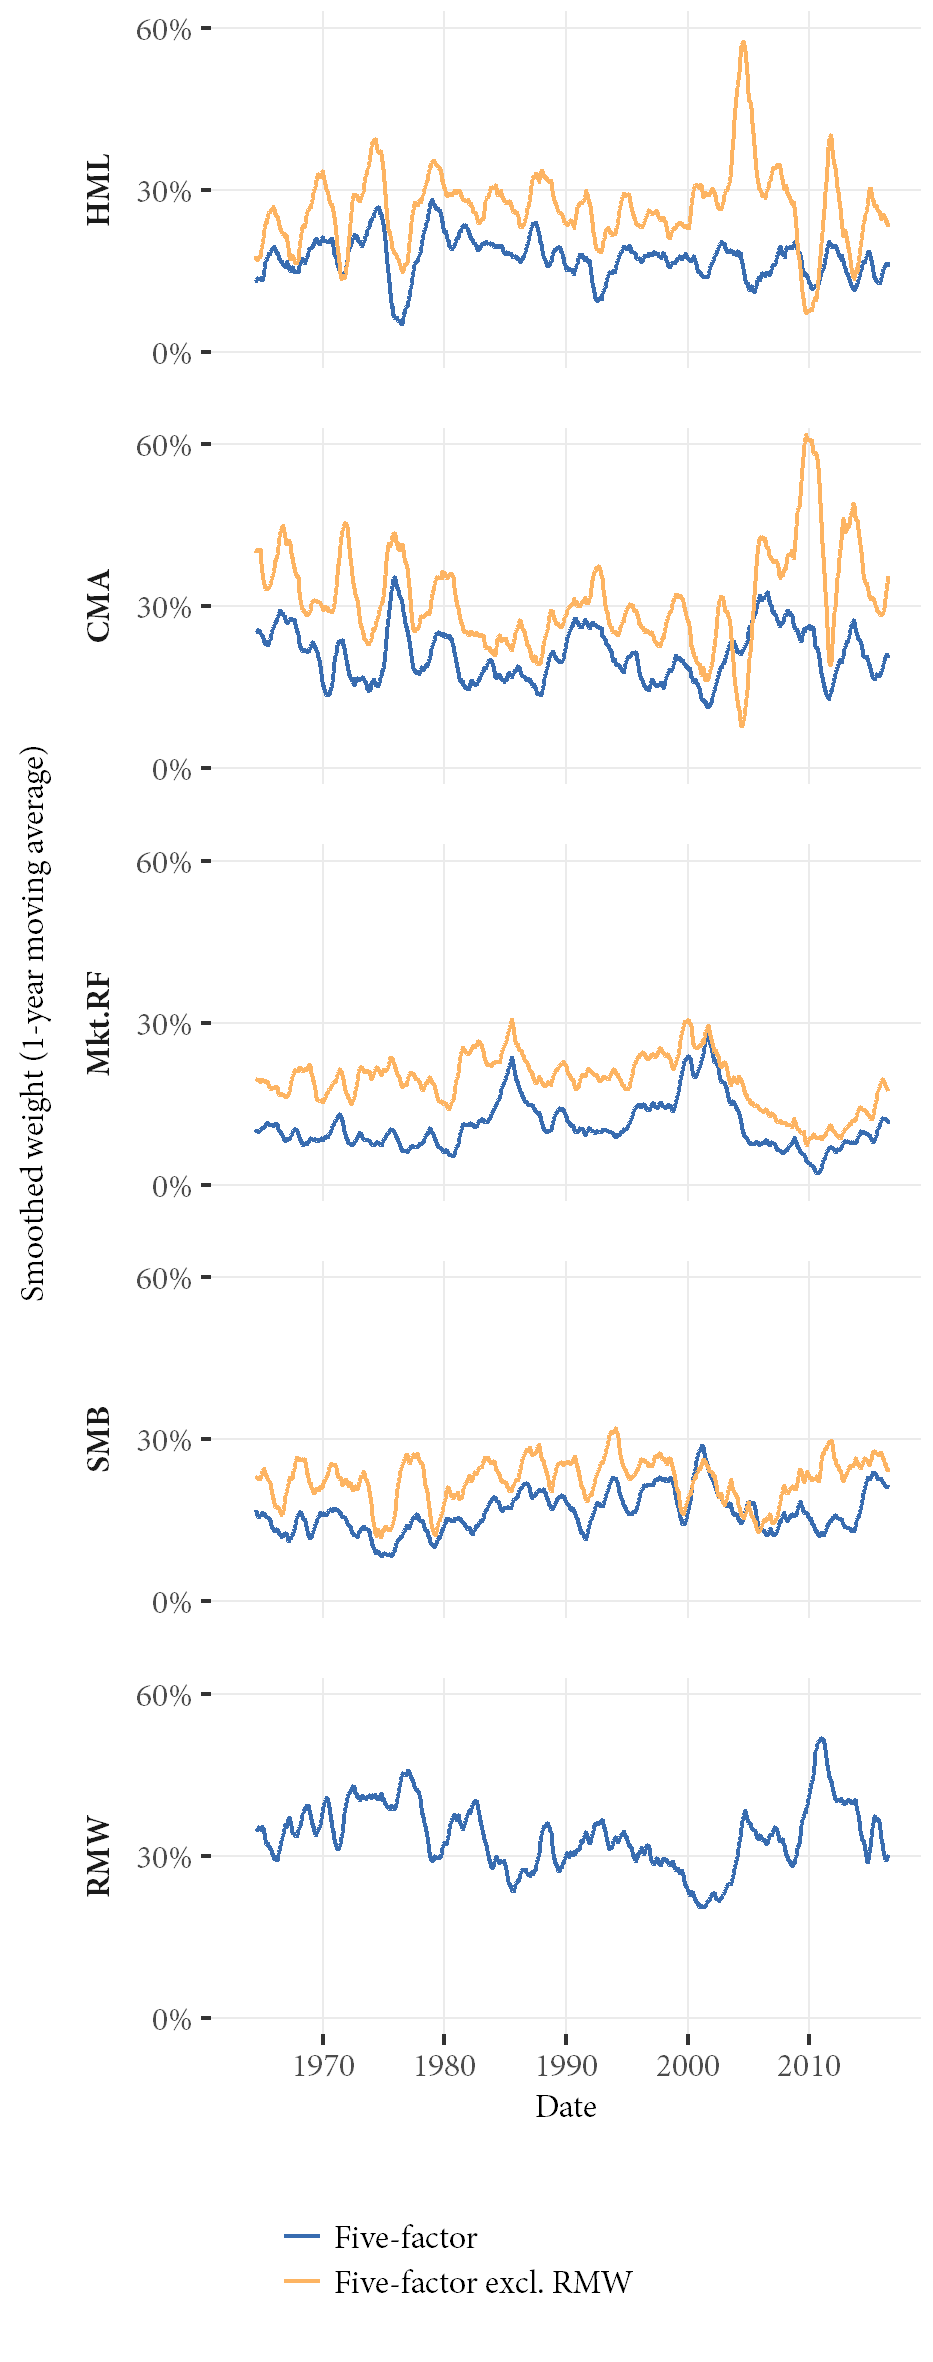
\includegraphics[scale=1]{graphics/weights/appendix_Weights_CDB_5F_5F_EXCL_RMW.png}
  \footnotesize
  \caption{CDB optimal weights with five factors (cont.)}
\end{figure}

\begin{figure}[htbp]
  \centering
  \footnotesize
  \begin{subfigure}{0.45\textwidth}

    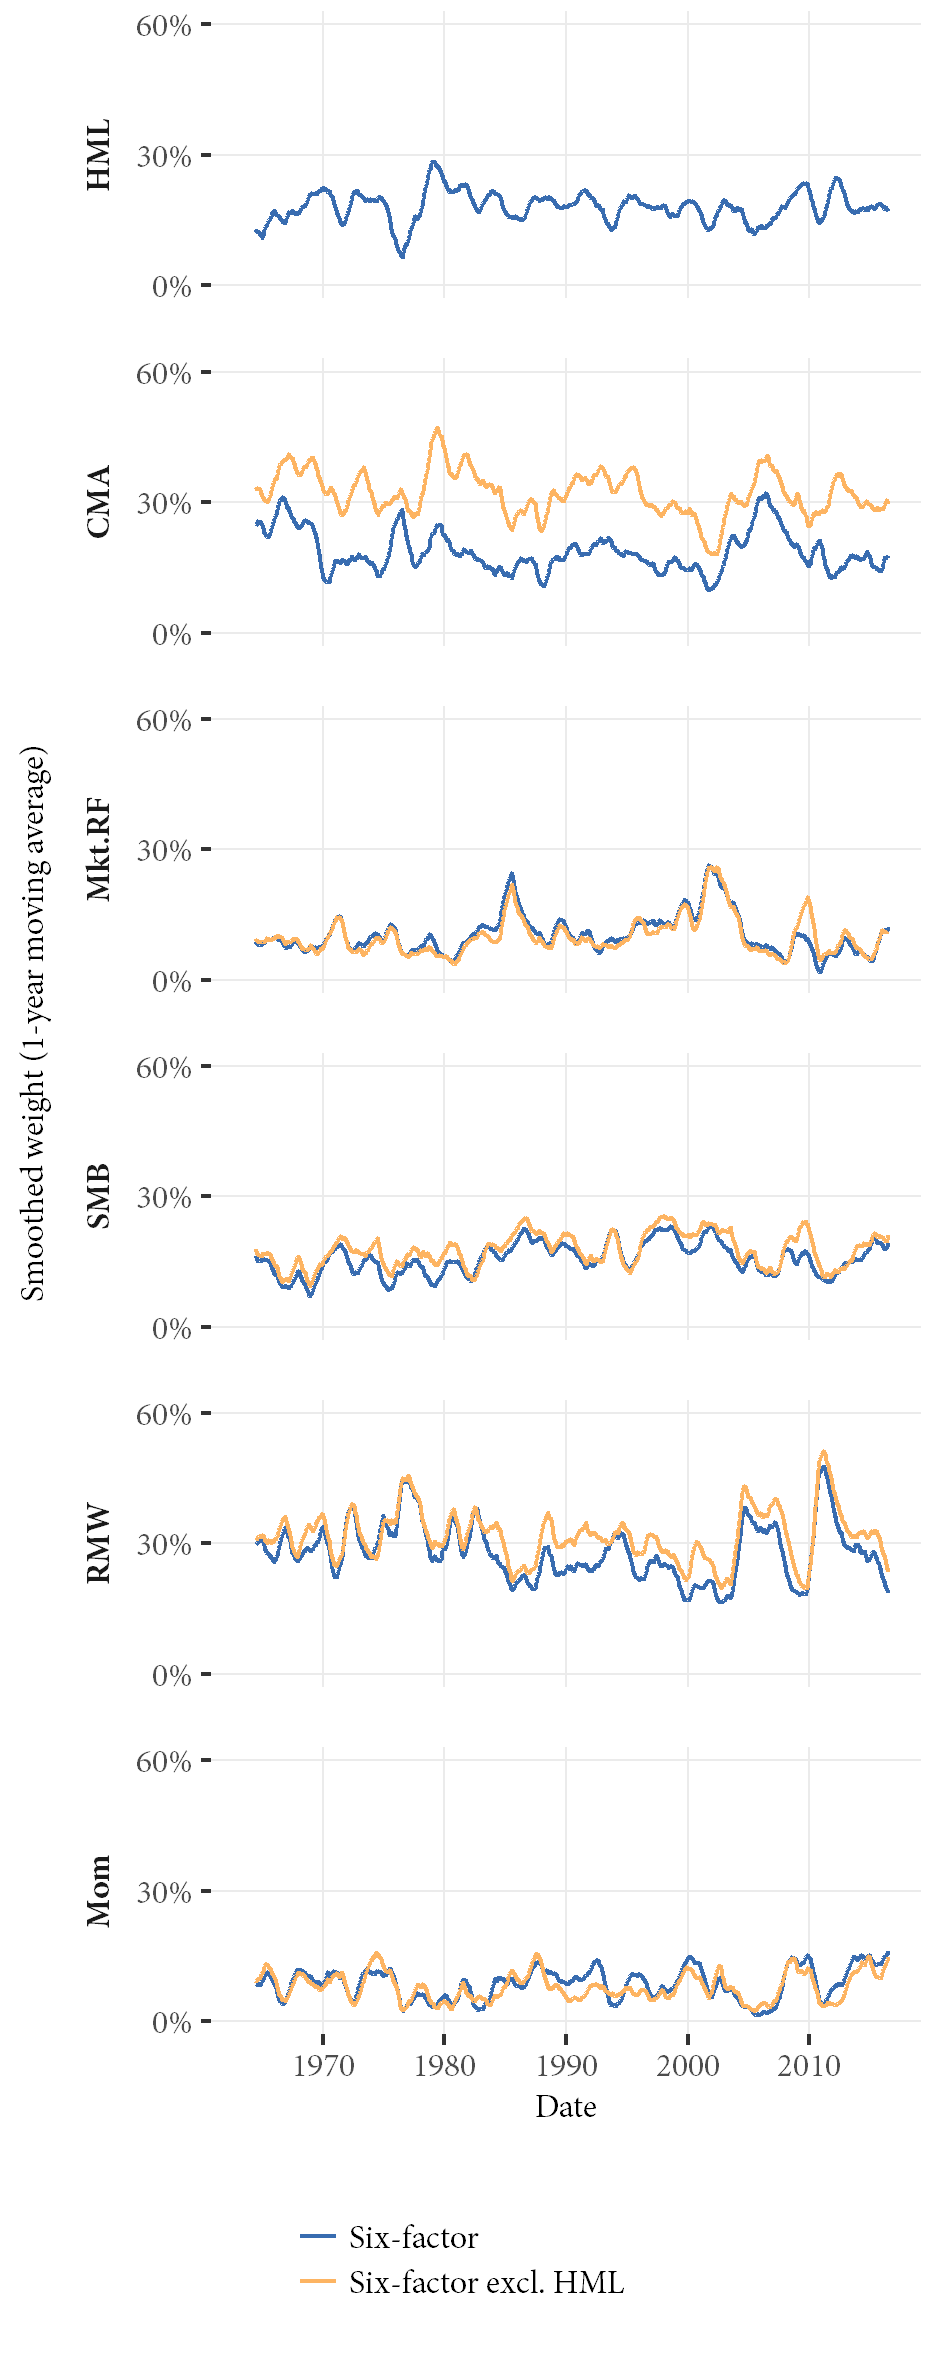
\includegraphics[width=\textwidth]{graphics/weights/appendix_Weights_CDB_6F_EXCL_HML_6F.png}
    \caption{Excluding HML}
  \end{subfigure}
  ~
  \begin{subfigure}{0.45\textwidth}
    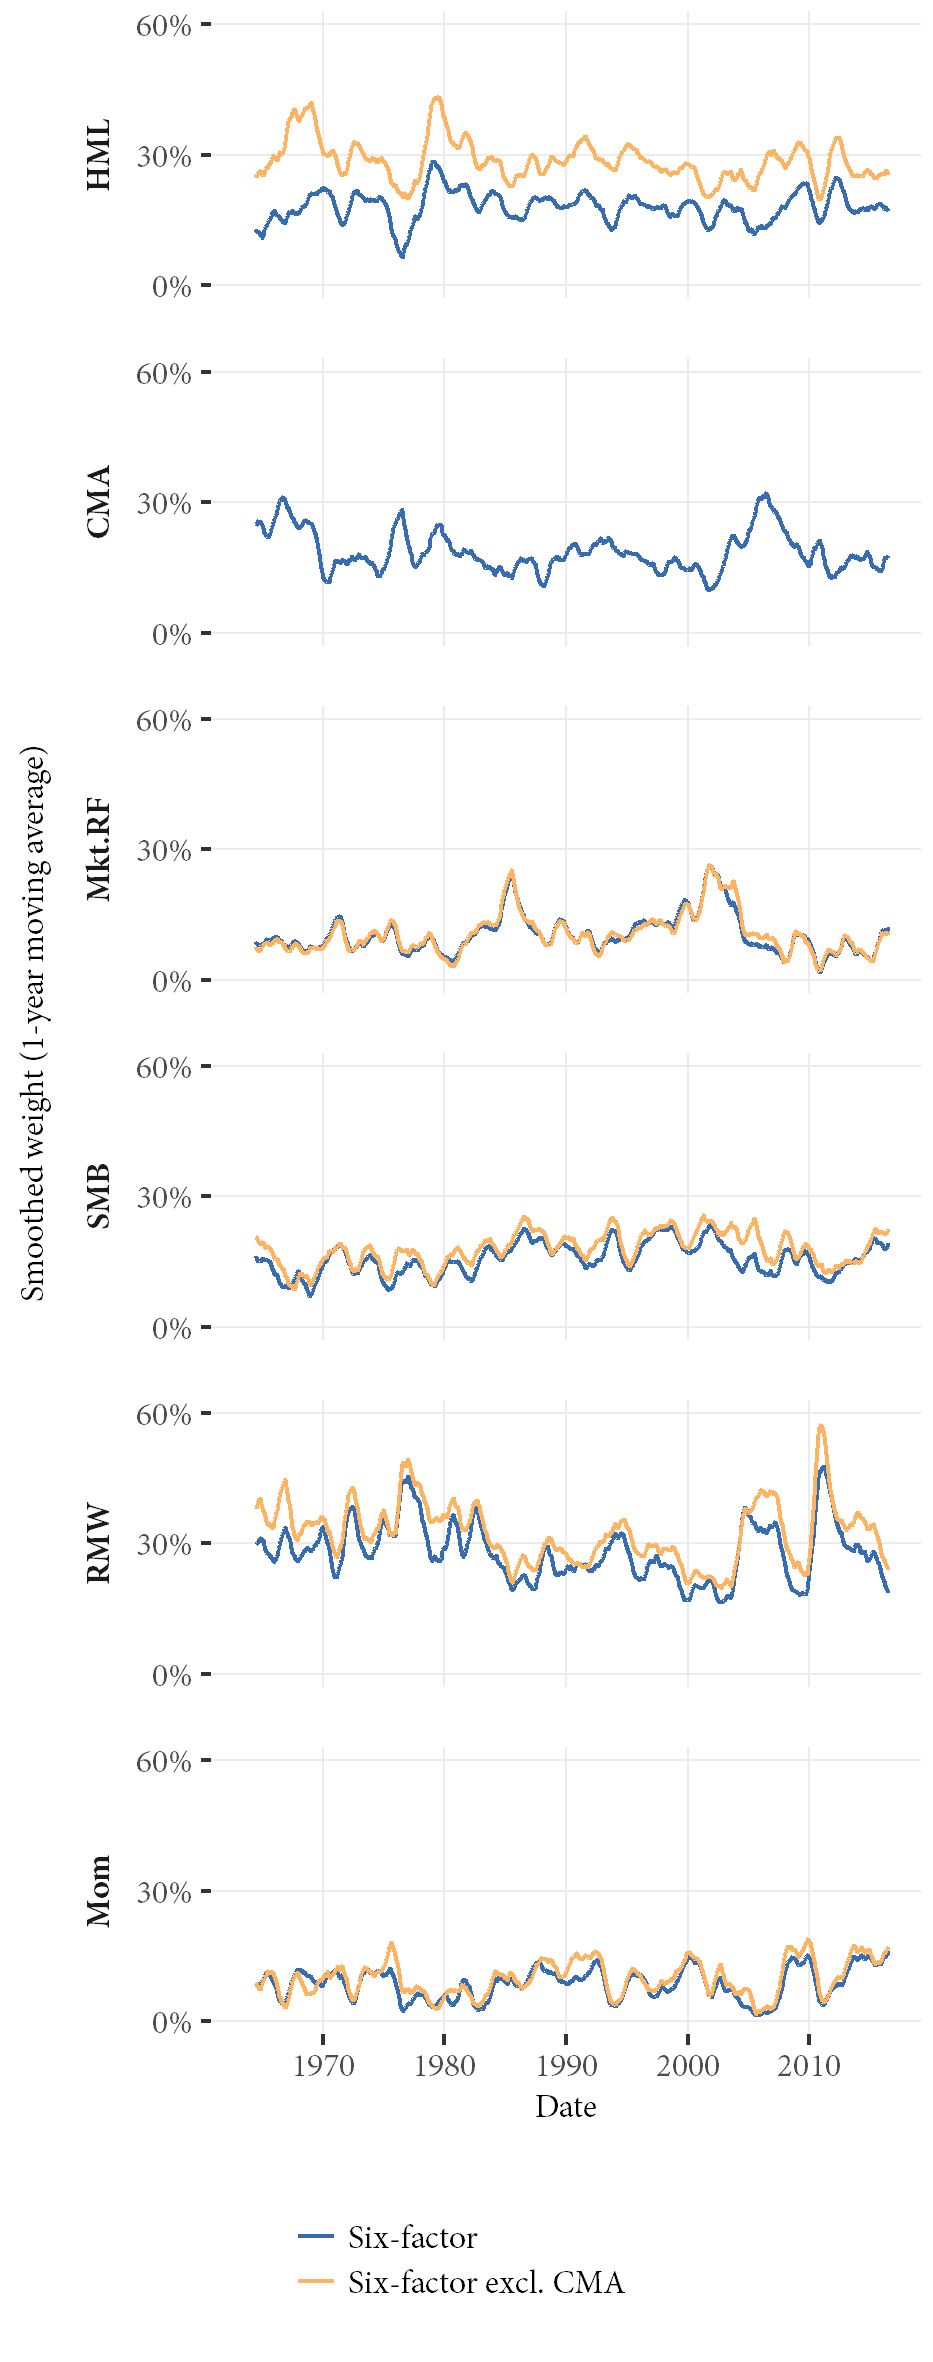
\includegraphics[width=\textwidth]{graphics/weights/appendix_Weights_CDB_6F_EXCL_CMA_6F.png}
    \caption{Excluding CMA}
  \end{subfigure}
  \caption{CDB optimal weights with six factors}

  \begin{longcaption}
    Smoothed as 1-year moving averages. Left hand panel including and excluding HML, right hand including and excluding CMA. Based on one-week-ahead forecasts from the copula model 1963--2016.
  \end{longcaption}
  \label{fig:cdb_optimal_6}
\end{figure}

\begin{figure}[htbp]
  \ContinuedFloat
  \centering
  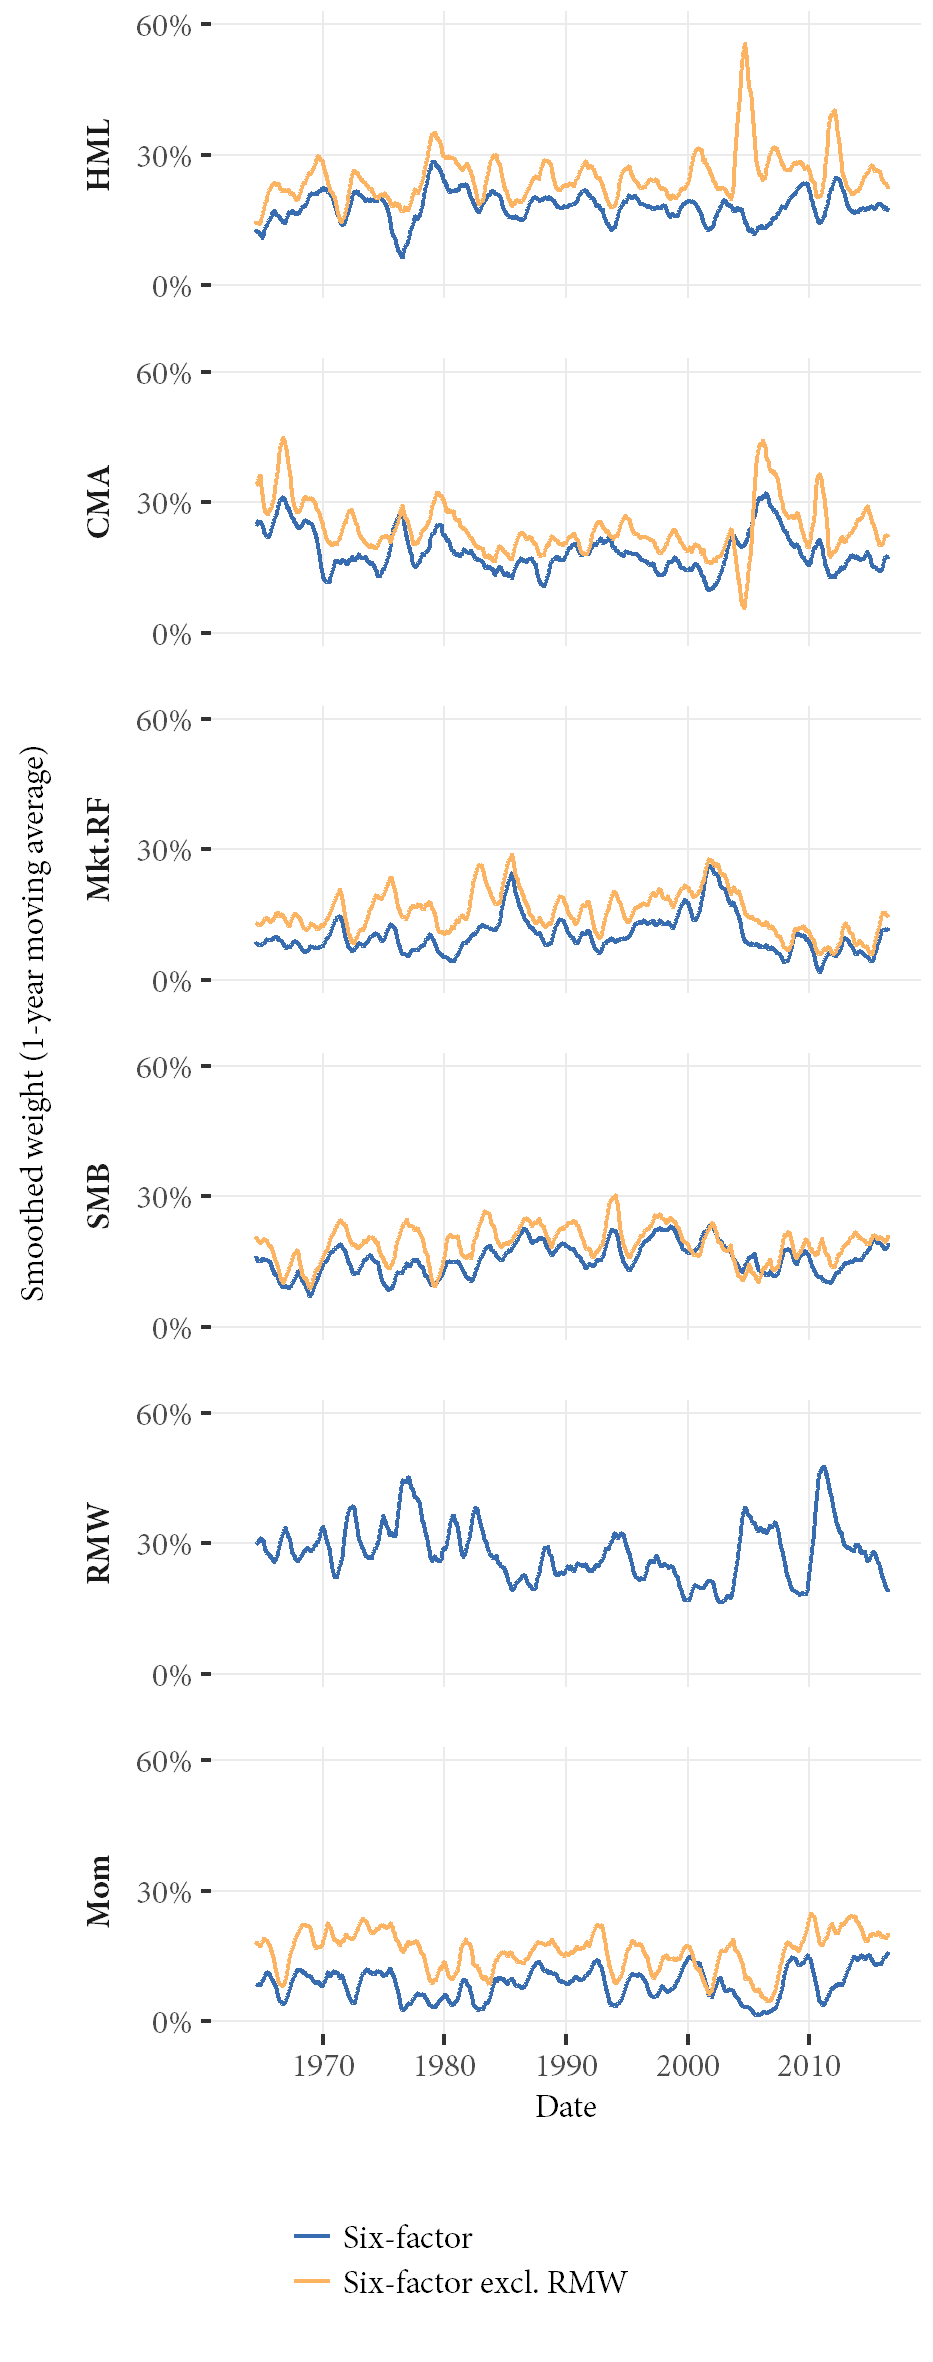
\includegraphics[scale=1]{graphics/weights/appendix_Weights_CDB_6F_6F_EXCL_RMW.png}
  \footnotesize
  \caption{CDB optimal weights with six factors (cont.)}
\end{figure}

% section supplementary_figures_and_tables (end)
